\documentclass[12pt, a4paper]{article}
\usepackage{ctex} % 支持中文处理
\usepackage{geometry} % 页面布局
\usepackage{graphicx} % 图片支持
\usepackage{hyperref} % 超链接支持
\usepackage{amsmath} % 数学公式
\usepackage{amsfonts}
\usepackage{amssymb}
\usepackage{amsthm}
\usepackage{bm}
\usepackage{color}
\usepackage{physics}
\newtheorem{lemma}{引理}
\newtheorem{theorem}{定理}
\geometry{left=2.5cm,right=2.5cm,top=2.5cm,bottom=2.5cm} % 设置页边距
\title{数理算法原理}
\author{安庭毅\ 工学院 \ 2100011014}
\date{\today} % 使用今天的日期

\begin{document}

\maketitle % 显示标题
\section{稳态等温线绘制}
取步长为0.3cm,松弛因子1.5,得到稳定的温度场如下图所示:
\begin{figure}[htbp]
    \centering
    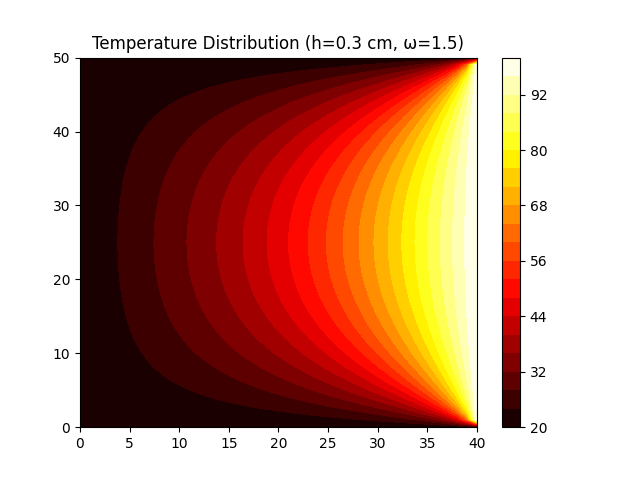
\includegraphics[width=\textwidth]{pictures/Temperature Distribution.png}
\end{figure}
\section{不同松弛因子收敛速率比较}
固定步长为1.5cm,收敛时的迭代步数随松弛因子变化如下图所示:
\begin{figure}[htbp]
    \centering
    \includegraphics[width=\textwidth]{pictures/Convergence vs. ω.png}
\end{figure}
可以看到迭代步数随松弛因子增加而先减少后增加。
\section{最优松弛因子比较}
取步长为1.5cm,1.0cm和0.5cm,分别通过数值计算和理论公式求出最优松弛因子,如下图所示:
\begin{figure}
    \centering
    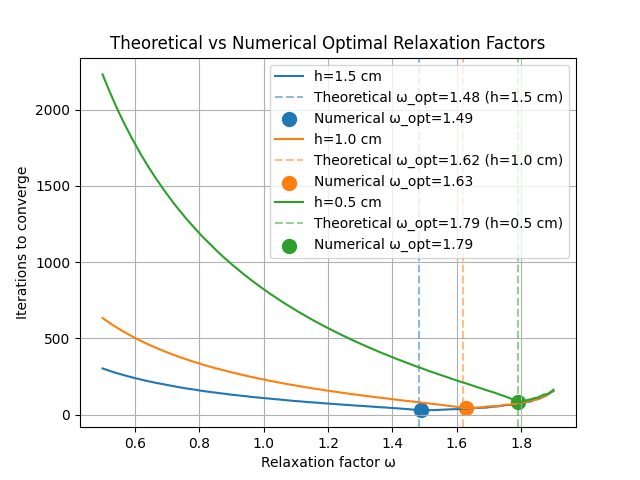
\includegraphics[width=\textwidth]{pictures/Theoretical vs Numerical Optimal Relaxation Factors.png}
\end{figure}
可以看到理论与数值计算结果良好吻合。

\section*{附1:AI工具使用说明表}
使用的AI工具:deepseek和GPT-4o

AI生成代码行数及功能:numerical\_test.py中32-37,47-53,74-83行由AI生成(有自主修改),均为画图功能

核心代码自主编写比例:62\%

\section*{附2:git版本控制记录}
\begin{figure}[htbp]
    \centering
    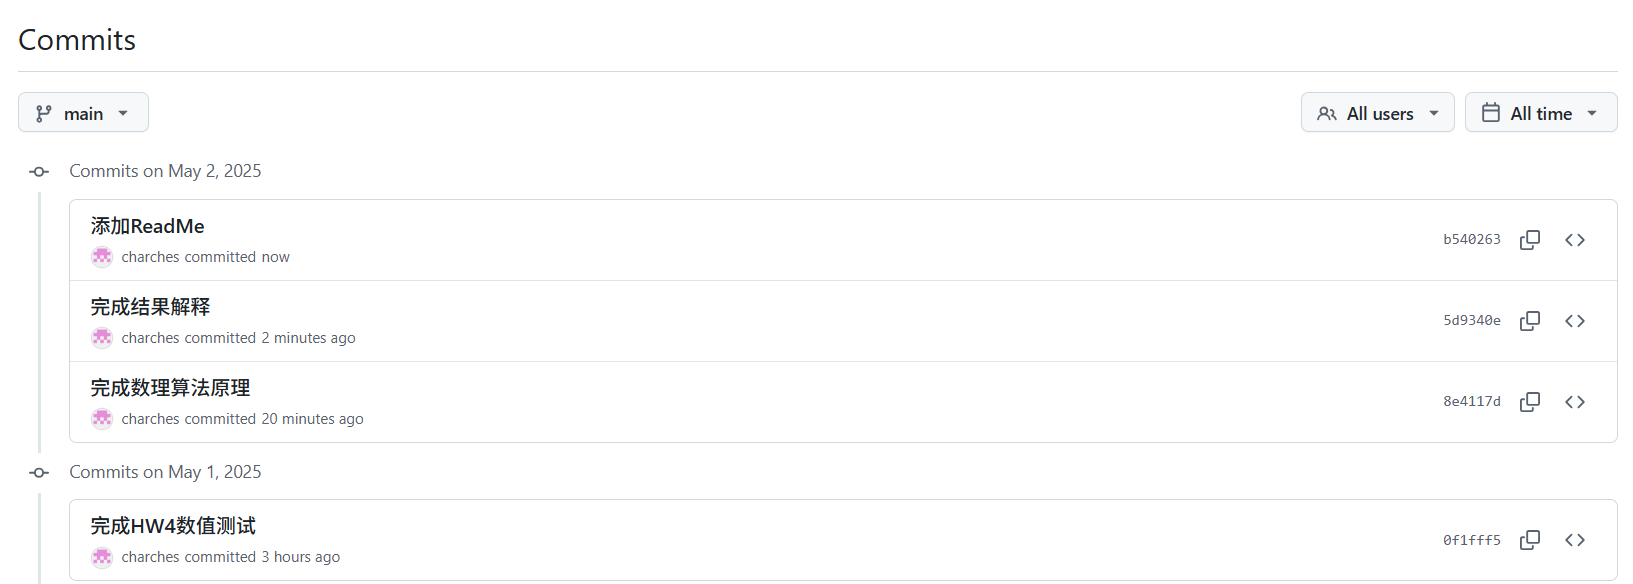
\includegraphics[width=0.8\textwidth]{./pictures/git_control.png}
\end{figure}
\end{document}
